\newpage
\section{Preventivo}
In questa sezione vengono presentati i grafici e le tabelle riassuntive per descrivere l'impegno previsto, in ore lavoro, dei diversi ruoli nei sei periodi sopra descritti. Inoltre viene mostrata una tabella riassuntiva al fine di rappresentare l'incidenza di ogni ruolo nell'intero progetto.

\subsection{\ARM}
Questa fase è considerata un investimento del \termine{team} per aggiudicarsi il progetto e per tale motivo non verrà rendicontata nel calcolo del preventivo. \\
Le ore impiegate in questo periodo sono 179 e vengono ripartite in:

\begin{table}[h]
	\begin{center}
		\begin{tabular}{|c|c|}
			\hline
			\textbf{Ruolo}	& \textbf{Ore} \\
			\hline
			\Pm &	20\\
			\hline
			\Am	&	19\\
			\hline
			\An		&	75\\
			\hline
			\Ver	&	65\\
			\hline
		\end{tabular}
	\end{center}
	\caption{Ore per ruolo, \ARM}
\end{table}

\begin{figure}[H]
	\centering 
	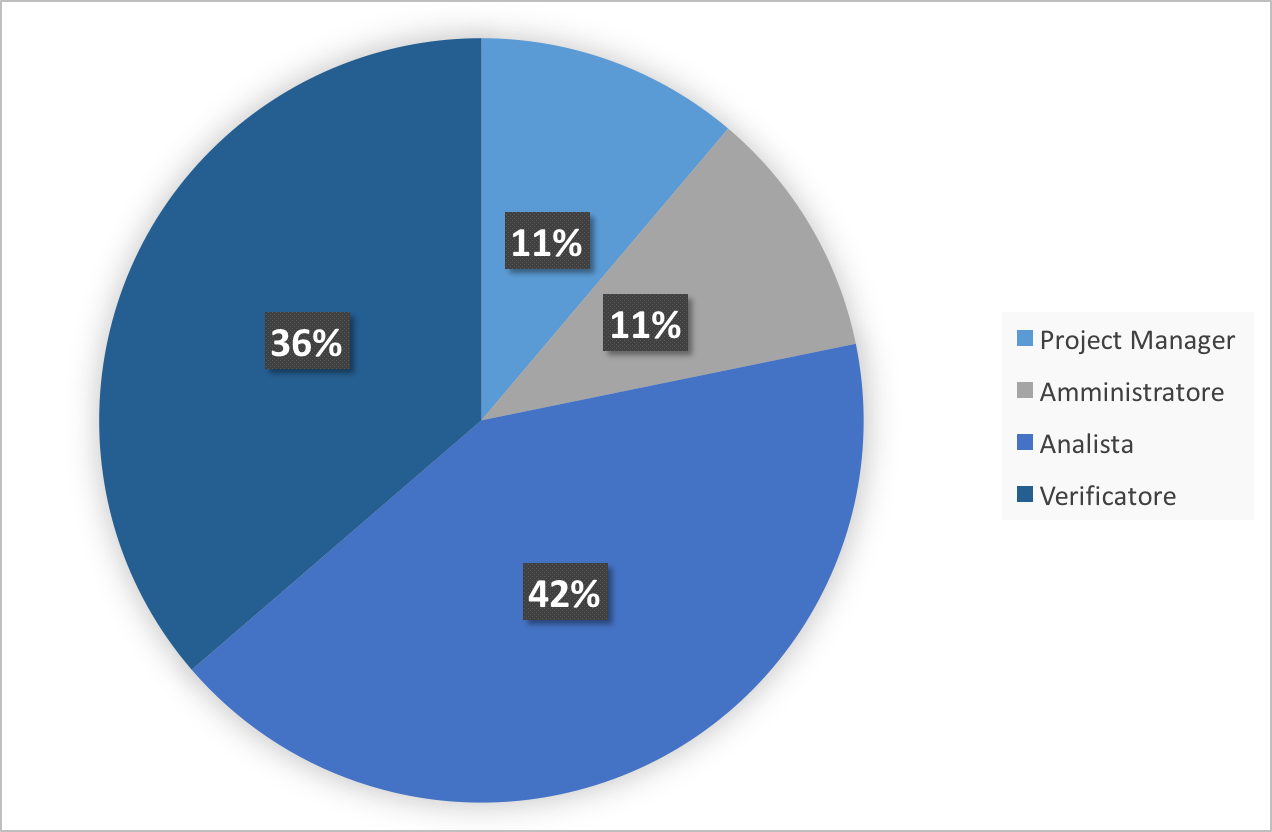
\includegraphics[scale=0.7]{Immagini/GraficiTorte/ARM.png}
	\caption{Ore per ruolo, \ARM}
\end{figure}

\newpage
\subsection{\ARD}
Le ore impiegate in questo periodo sono 50 e vengono ripartite in:

\begin{table}[h]
	\begin{center}
		\begin{tabular}{|c|c|}
			\hline
			\textbf{Ruolo}	& \textbf{Ore} \\
			\hline
			\Pm &	3\\
			\hline
			\Am	&	3\\
			\hline
			\An		&	30\\
			\hline
			\Ver	&	14\\
			\hline
		\end{tabular}
	\end{center}
	\caption{Ore per ruolo, \ARD}
\end{table}

\begin{figure}[H]
	\centering 
	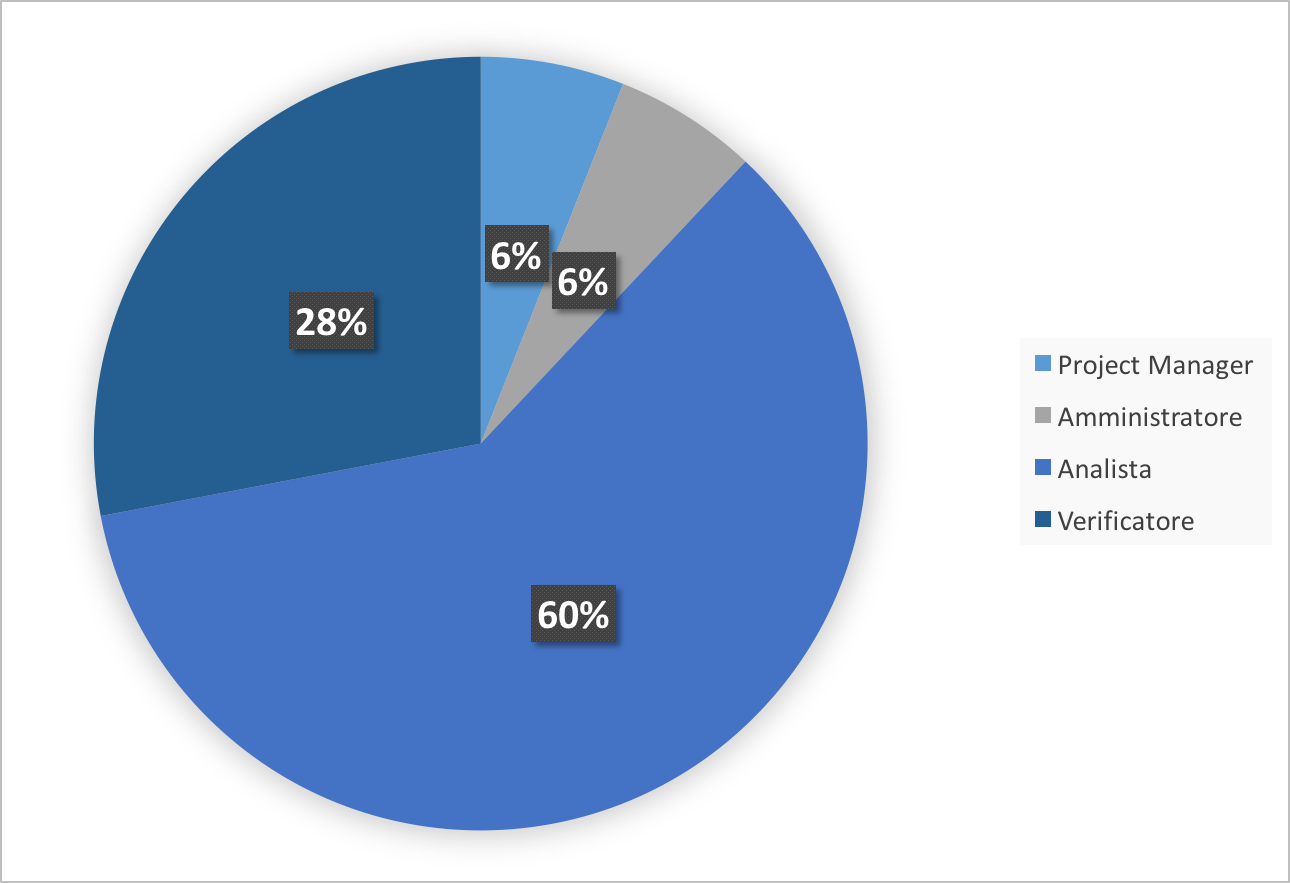
\includegraphics[scale=0.7]{Immagini/GraficiTorte/ARD.png}
	\caption{Ore per ruolo, \ARD}
\end{figure}
\newpage
\subsection{\PA}
Le ore totali impiegate in questo periodo sono 198 e vengono ripartite in:

\begin{table}[h]
	\begin{center}
		\begin{tabular}{|c|c|}
			\hline
			\textbf{Ruolo}	& \textbf{Ore} \\
			\hline
			\Pm &	6\\
			\hline
			\Am	& 7\\
			\hline
			\Prog & 120\\
			\hline
			\Ver	&	65\\
			\hline
		\end{tabular}
	\end{center}
	\caption{Ore per ruolo, \PA}
\end{table}

\begin{figure}[H]
	\centering 
	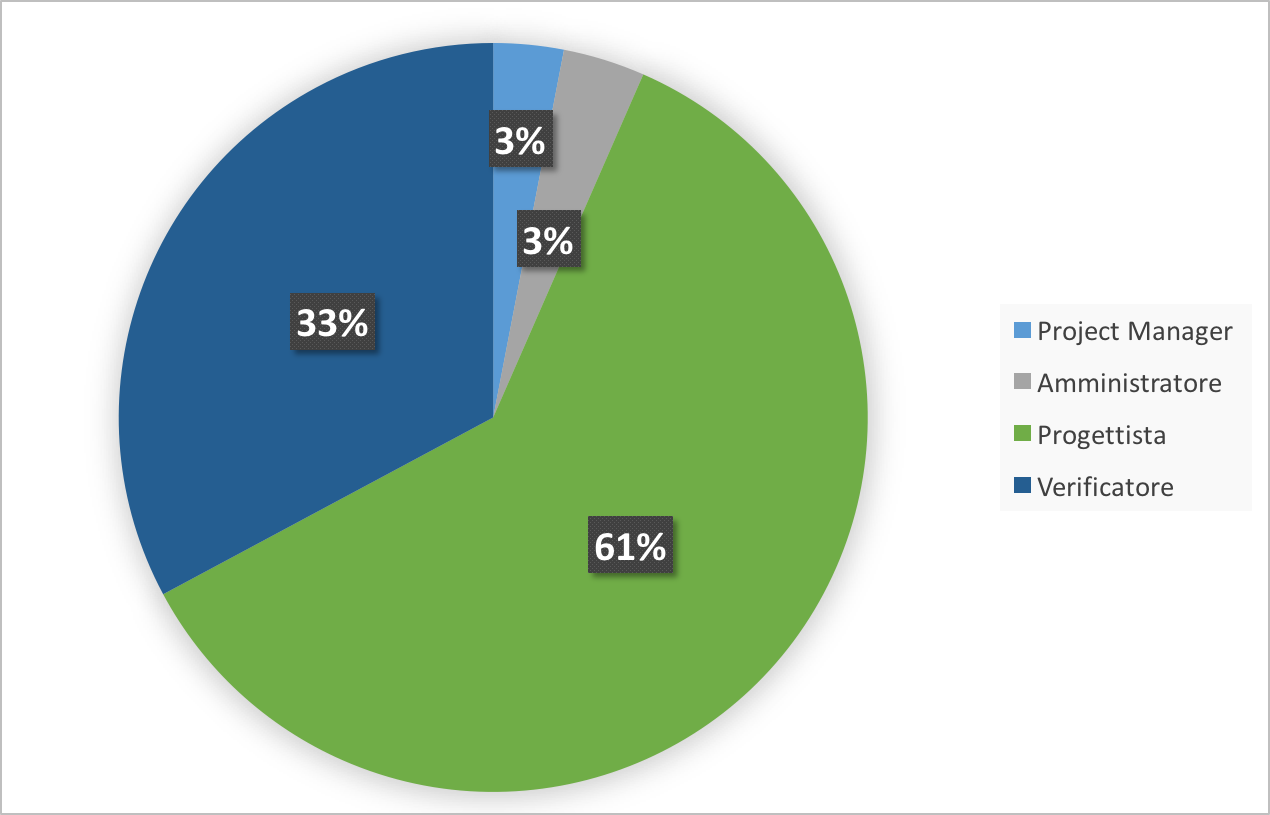
\includegraphics[scale=0.7]{Immagini/GraficiTorte/PA.png}
	\caption{Ore per ruolo, \PA}
\end{figure}

\newpage
\subsection{\PD\ e \COD}
Le ore totali impiegate in questo periodo sono 443 e vengono ripartite in:

\begin{table}[h]
	\begin{center}
		\begin{tabular}{|c|c|}
			\hline
			\textbf{Ruolo}	& \textbf{Ore} \\
			\hline
			\Pm &	18\\
			\hline
			\Am	&	13\\
			\hline
			\Prog	&	86\\
			\hline
			\Progr	&	137\\
			\hline
			\Ver	&	119\\
			\hline
		\end{tabular}
	\end{center}
	\caption{Ore per ruolo, \PD\ e \COD}
\end{table}

\begin{figure}[H]
	\centering 
	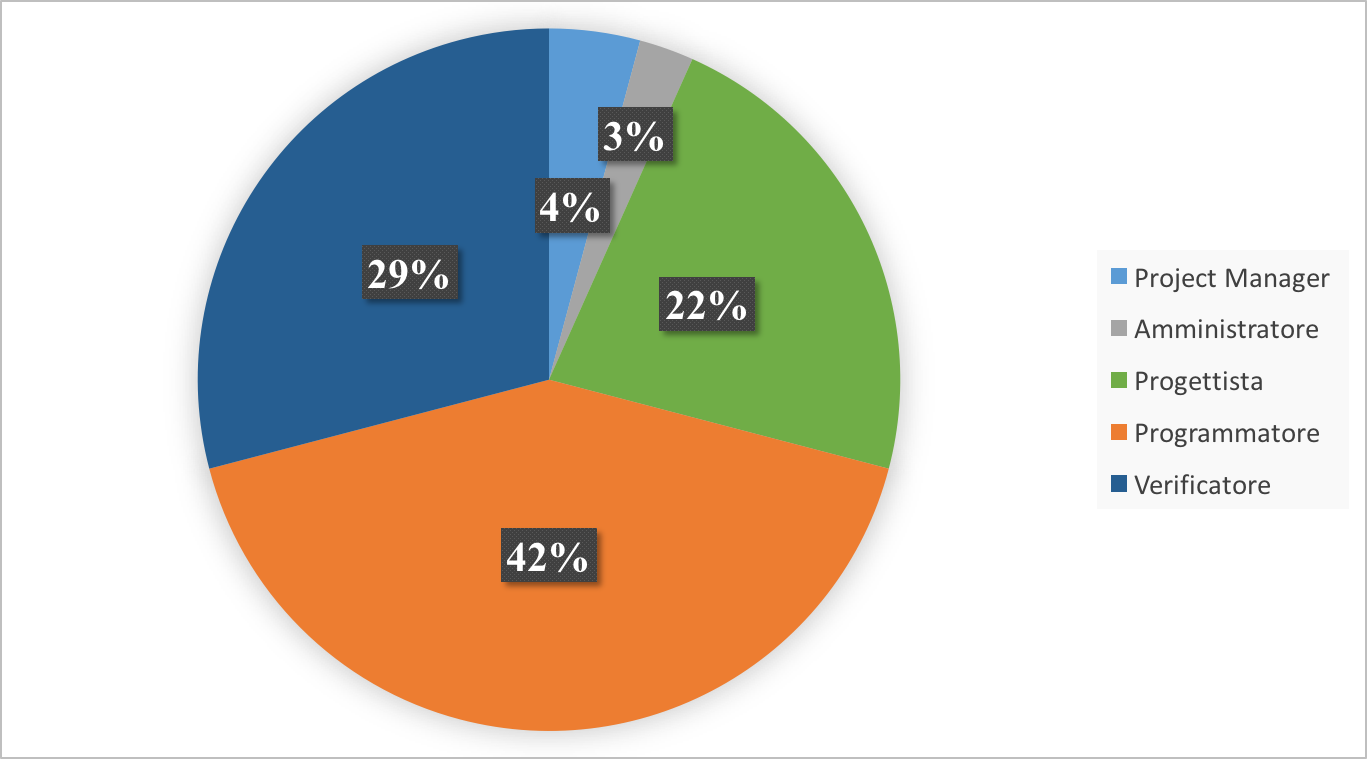
\includegraphics[scale=0.7]{Immagini/GraficiTorte/PDCOD.png}
	\caption{Ore per ruolo, \PD\ e \COD}
\end{figure}

\newpage
Fino alla \RP\ sono state pianificate 121 delle ore descritte in precedenza suddivise come segue:

\begin{table}[h]
	\begin{center}
		\begin{tabular}{|c|c|}
			\hline
			\textbf{Ruolo}	& \textbf{Ore} \\
			\hline
			\Pm &	7\\
			\hline
			\Am	&	7\\
			\hline
			\Prog	&	65\\
			\hline
			\Ver	&	42\\
			\hline
		\end{tabular}
	\end{center}
	\caption{Ore per ruolo, \PD\ e \COD\ fino a \RP}
\end{table}

\begin{figure}[H]
	\centering 
	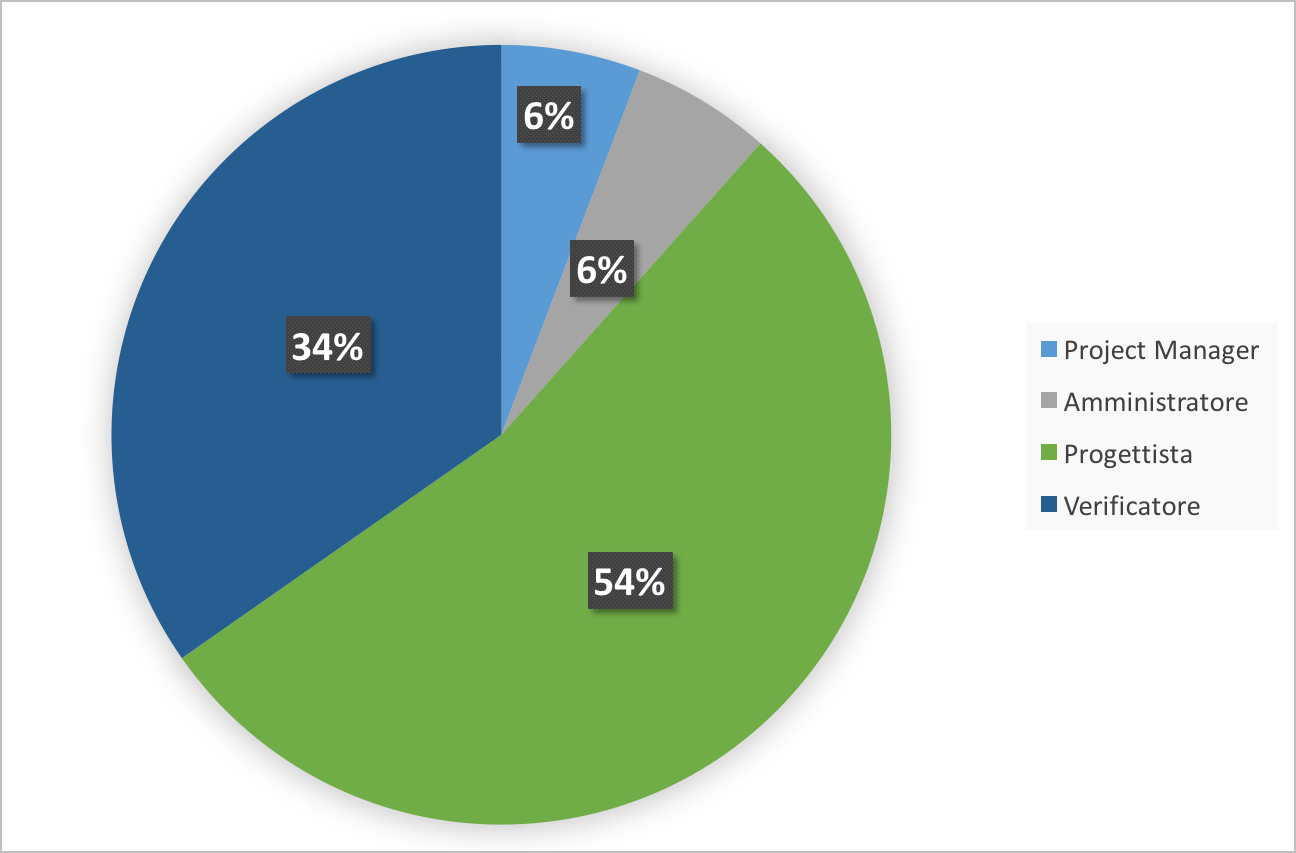
\includegraphics[scale=0.7]{Immagini/GraficiTorte/PD.png}
	\caption{Ore per ruolo, \PD\ e \COD\ fino a \RP}
\end{figure}

\newpage
Mentre dalla \RP\ fino al termine coincidente con la consegna per la \RQ\ le 322 ore rimanenti sono suddivise come segue:

\begin{table}[h]
	\begin{center}
		\begin{tabular}{|c|c|}
			\hline
			\textbf{Ruolo}	& \textbf{Ore} \\
			\hline
			\Pm &	11\\
			\hline
			\Am	&	6\\
			\hline
			\Prog	&	21\\
			\hline
			\Progr	&	193\\
			\hline
			\Ver	&	91\\
			\hline
		\end{tabular}
	\end{center}
	\caption{Ore per ruolo, \PD\ e \COD\ da \RP\ fino a \RQ}
\end{table}

\begin{figure}[H]
	\centering 
	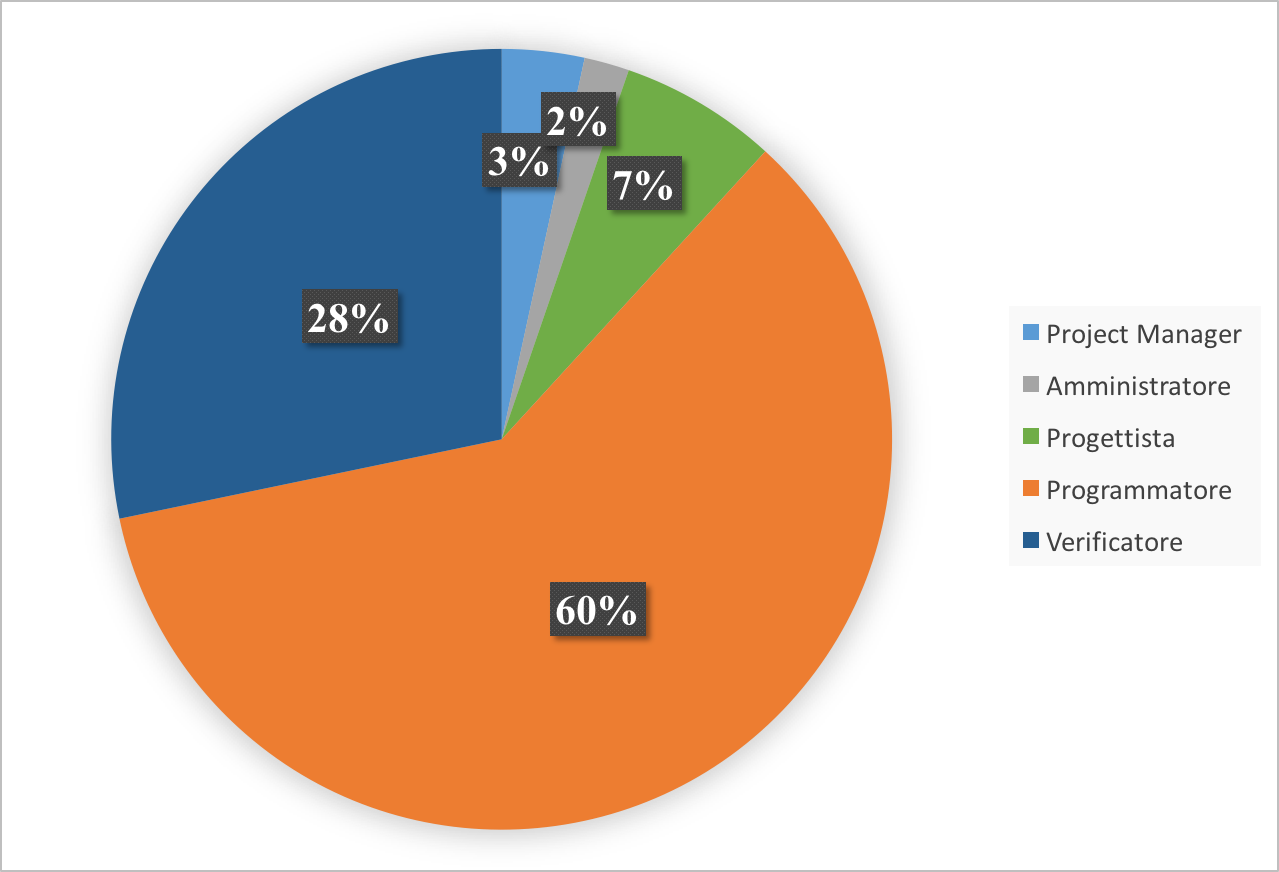
\includegraphics[scale=0.7]{Immagini/GraficiTorte/COD.png}
	\caption{Ore per ruolo, \PD\ e \COD\ da \RP\ fino a \RQ}
\end{figure}

Le ore di questo periodo di \PD\ e \COD\ includono anche 70 ore di autoapprendimento. Infatti, dato il verificarsi del rischio tecnologico relativo alla difficile comprensione di alcune tecnologie, in particolare la difficile comprensione della documentazione della piattaforma \termine{Rocket.chat}, sono state previste ulteriori ore di autoapprendimento per i ruoli di \Progr\ e \Ver\ suddivise come segue:

\begin{table}[h]
	\begin{center}
		\begin{tabular}{|c|c|}
			\hline
			\textbf{Ruolo}	& \textbf{Ore} \\
			\hline
			\Progr	&	56\\
			\hline
			\Ver	&	14\\
			\hline
		\end{tabular}
	\end{center}
	\caption{Ore di autoapprendimento per ruolo, \PD\ e \COD\ da \RP\ fino a \RQ}
\end{table}

Le ore di autoapprendimento, come le ore di investimento iniziale, non verranno rendicontate nel calcolo del preventivo.

\newpage
\subsection{\VV}
Le ore totali in questo periodo sono 114 e vengono ripartite in:

\begin{table}[h]
	\begin{center}
		\begin{tabular}{|c|c|}
			\hline
			\textbf{Ruolo}	& \textbf{Ore} \\
			\hline
			\Pm &	14\\
			\hline
			\Am	&	8\\
			\hline
			\Prog		&	12\\
			\hline
			\Progr & 11\\
			\hline
			\Ver	&	69\\
			\hline
		\end{tabular}
	\end{center}
	\caption{Ore per ruolo, \VV}
\end{table}

\begin{figure}[H]
	\centering 
	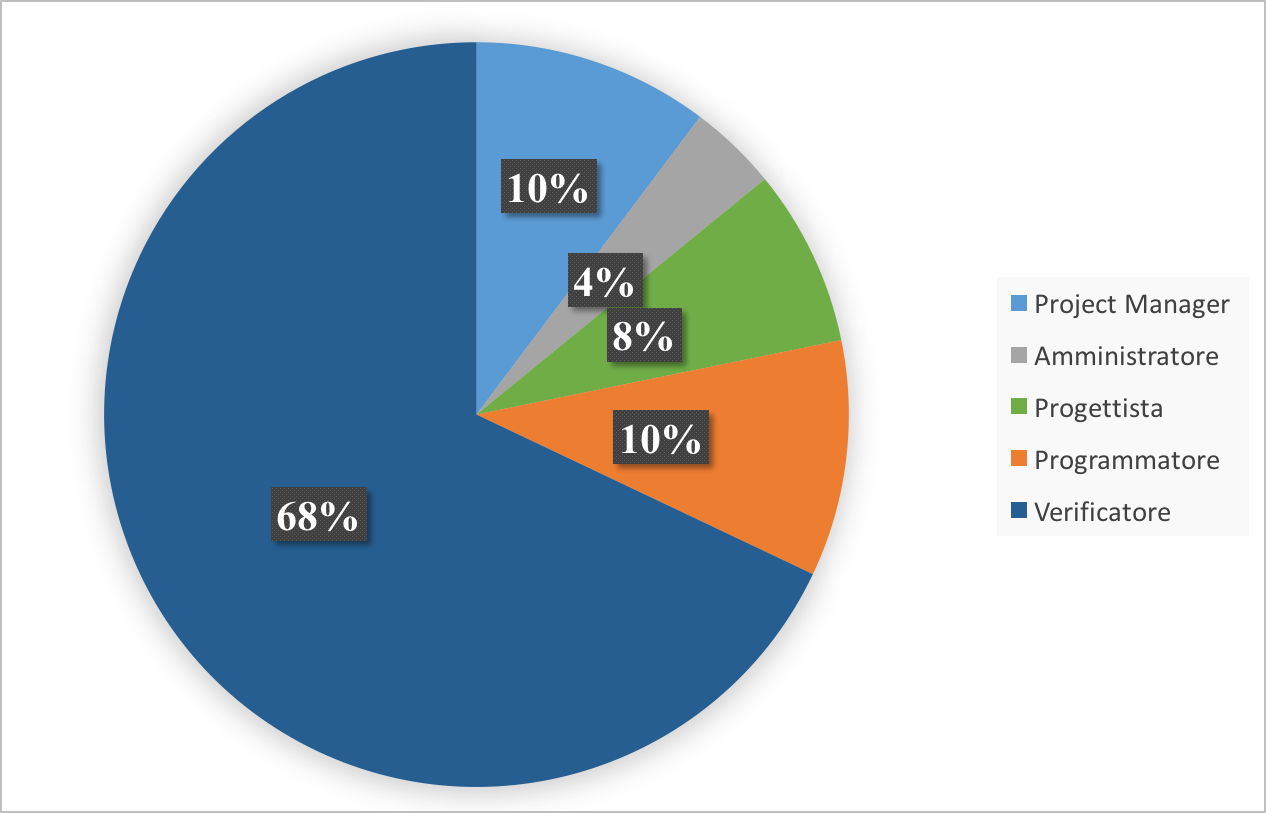
\includegraphics[scale=0.7]{Immagini/GraficiTorte/VV.png}
	\caption{Ore per ruolo, \VV}
\end{figure}
\newpage
\subsection{Quadro riassuntivo}
Le ore totali del progetto sono 984, di cui 735 remunerabili, così ripartite:

\begin{table}[h]
	\begin{center}
		\begin{tabular}{|c|c|c|}
			\hline
			\textbf{Ruolo}	& \textbf{Ore totali} & \textbf{Ore remunerabili} \\
			\hline
			\Pm &	61	&	41	\\
			\hline
			\Am	&	50	&	31	\\
			\hline
			\An		&	105	&	30	\\
			\hline
			\Prog		&	218	&	218	\\
			\hline
			\Progr	&	218	&	148	\\
			\hline
			\Ver	&	346	&	267	\\
			\hline
		\end{tabular}
	\end{center}
	\caption{Ore per ruolo, Quadro riassuntivo}
\end{table}

\begin{figure}[H]
	\centering 
	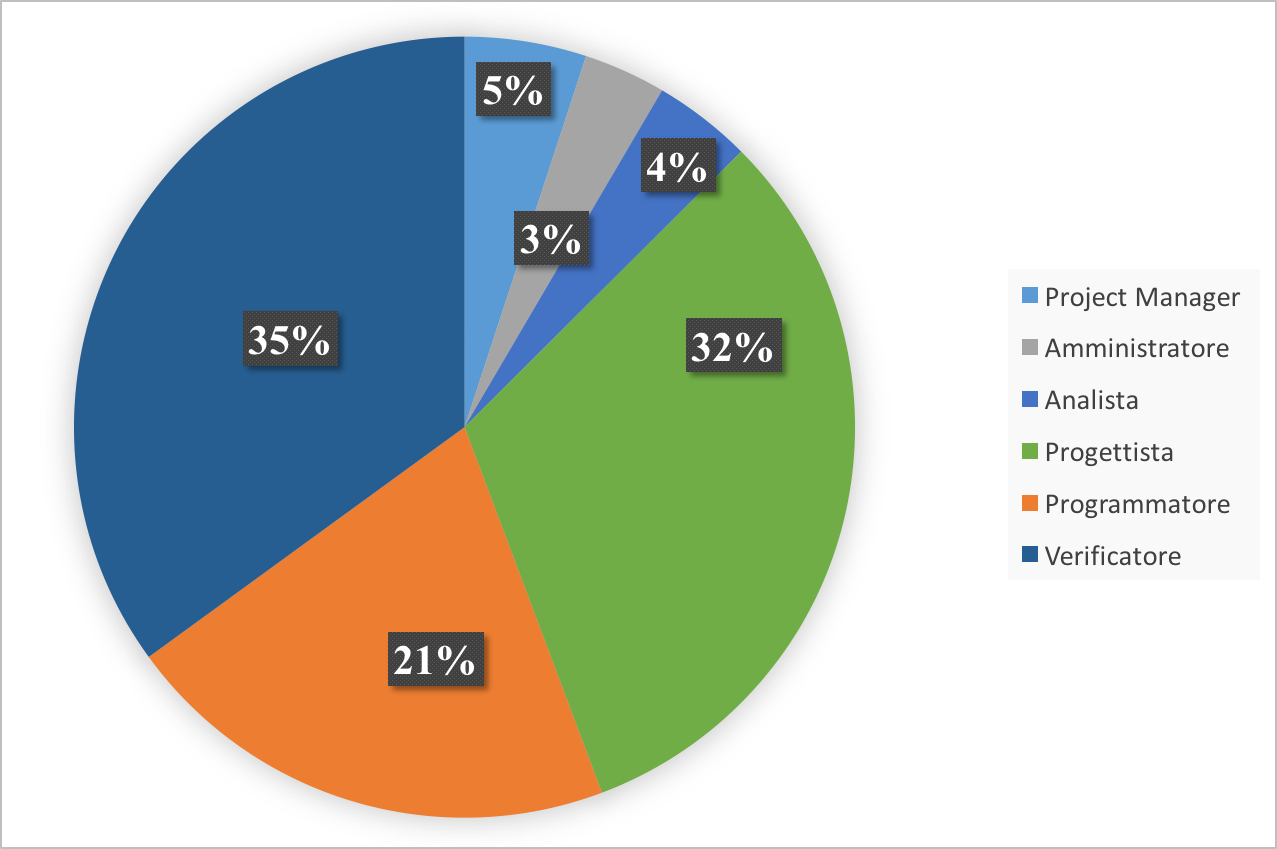
\includegraphics[scale=0.7]{Immagini/GraficiTorte/TOT.png}
	\caption{Ore totali per ruolo}
\end{figure}